\documentclass[tikz,border=10pt]{standalone}
\usepackage{amsmath}

\tikzset{
    axis/.style={->,thick},
    sphere/.style={draw=blue!50,fill=blue!20,opacity=0.7},
    rt-surface/.style={draw=red,dashed}
}

\begin{document}
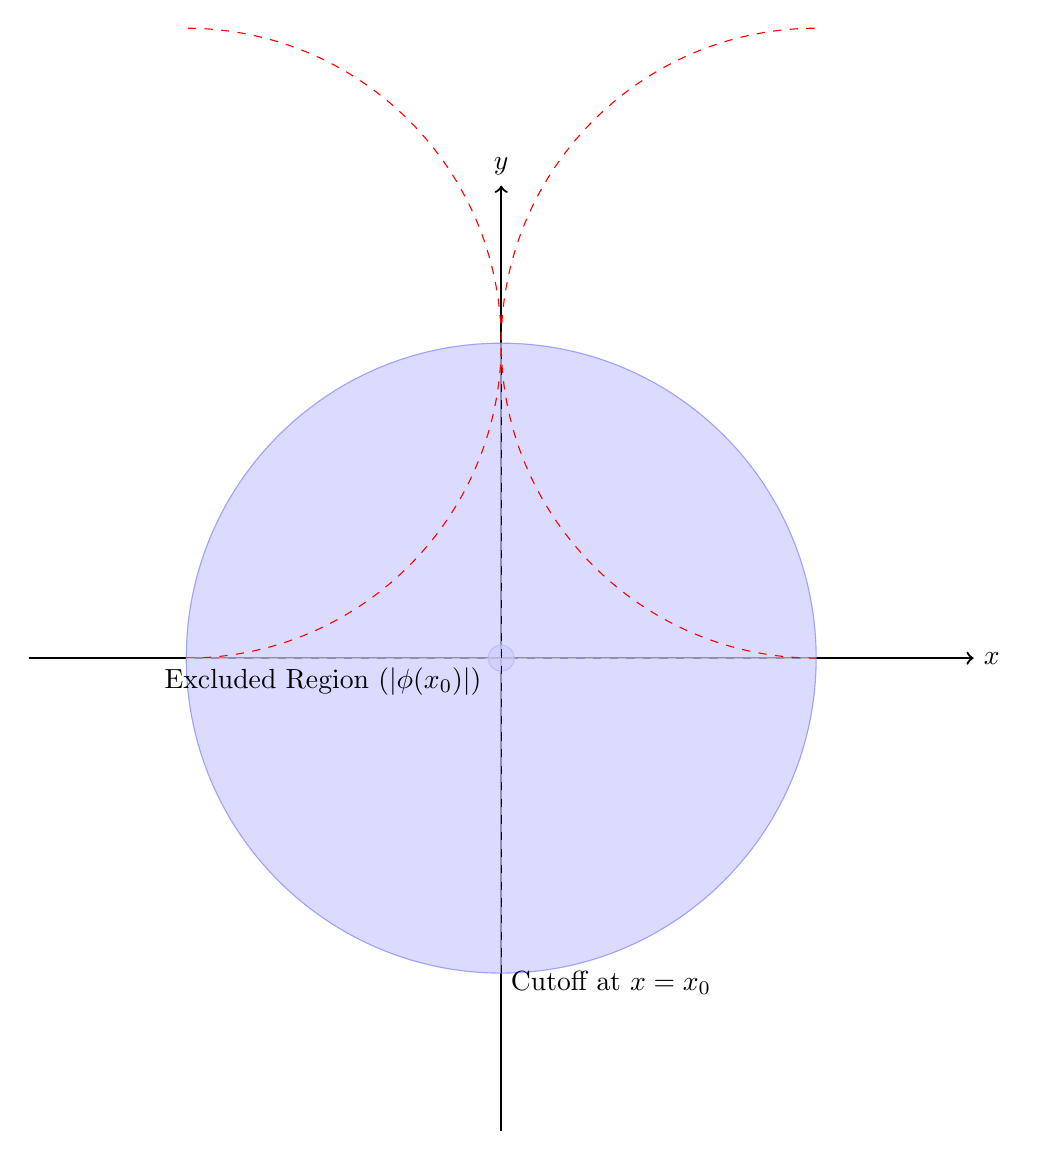
\begin{tikzpicture}[scale=2]
    % Axes
    \draw[axis] (-3,0) -- (3,0) node[right] {$x$};
    \draw[axis] (0,-3) -- (0,3) node[above] {$y$};

    % Sphere
    \node[circle,sphere] (sphere) at (0,0) {};
    \draw[sphere] (0,0) circle (2cm);

    % Cutoff line
    \draw[dashed] (0,-2) -- (0,2);
    \node[anchor=south west] at (0,-2.2) {Cutoff at $x = x_0$};

    % RT Surface
    \draw[rt-surface] (-2,0) arc[start angle=-90,end angle=90,radius=2cm];
    \draw[rt-surface] (2,0) arc[start angle=270,end angle=90,radius=2cm];

    % Excluded region
    \draw[dashed,gray!50] (-2,0) -- (2,0);
    \node[anchor=north west] at (-2.2,0) {Excluded Region ($|\phi(x_0)|$)};
\end{tikzpicture}
\end{document}